\chapter{Antenna theory}
So far we have cruised through understanding electromagnetic waves and not how they were generated. Now it is of concern to us and we ask the question of how electromagnetic waves are generated. In this chapter we will be answering that question through the topic called radiation. 

Essentially this chapter deals first with the principles of generation of electromagnetic waves and then practical devices which can generate electromagnetic waves from currents and voltages and also convert the electromagnetic waves to currents and voltages- which is called an \textbf{Antenna}\index{antenna}.

\section{Radiation}
The basis of radiation is the \textbf{accelerated charges}. From electrostatics, when there is a charge, then there is essentially electric field. If the charge is kept in motion, then it constitute current and current produces magnetic field but this current is in uniform motion. However what happens when there is time varying current (a current which varies as a function of time and therefore it gets accelerated and decelerated), what kind of field would exist? Well, the answer is simple, as stated earlier, accelerated charges is the basis of radiation and radiation is the propagation of electromagnetic field.

However, every accelerated charge may not give you radiation because if it would, a simple coaxial cable having time varying currents should produce radiation but that is not what happens. Well one other condition has to be satisfied. Lets consider a transmission line as shown below for the example we considered earlier - a coaxial cable - where the distance between the lines is far less than the wavelength of the time varying signal flowing through the transmission line.
\begin{figure}[h]
\centering
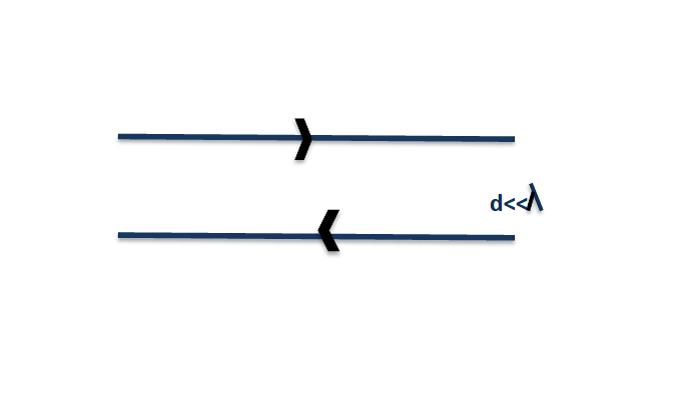
\includegraphics[height=5cm]{./graphics/fig_1}
\caption{Transmission line}
\end{figure}

As discussed in the previous chapter, the transmission line completely guides the electromagnetic energy within its structure. This can be understood from the current standing wave equation given by
$$I(l)=\dfrac{V^+}{Z_o}e^{-\gamma l} - \dfrac{V^-}{Z_o}e^{-\gamma l}$$
The components of the equation shows that the traveling currents are traveling in opposite direction as shown in fig 1.1. Essentially the field produced by each of the time varying components cancel out because the distance between the lines is extremely small (d$\ll\lambda$). 

So though we have accelerated and decelerated charges, we do not have radiation. However we can say that there is a possibility of radiation because accelerated and decelerated charges are capable of giving radiation. However if the distance between the lines in fig 1.1 are separated further such that $d\approx\lambda$ as shown in fig 1.2, then the cancellation will not take place in all direction. For instance if it cancels in one direction, in some other direction it is possible that phase of the wave is changed due to phase difference between propagating waves of the two currents and there might be radiation from the structure.
Therefore, it appears that radiation has two conditions which are; 
\begin{enumerate}[(i)]
\item There must be time varying currents; and
\item There must be spatial imbalance of the currents.
\end{enumerate}
Now lets identify structures where these conditions are clearly specified.

\subsection{RADIATION PHENOMENA}
With these points it is important to note that as frequency increases, the acceleration and deceleration of charges will increase because the rate at which the current is changing is higher. Hence as frequency increase for the same amplitude of currents, same peak current or RMS current, we should get more radiation. What we have designed in fig1.2b is essentially an antenna; and in designing any antenna, we will want the structure to give radiation effectively, also we will want the structure to transfer sufficient amount of power in the form of EM waves which will take the power away from the structure.

Just as an illustration we take a transmission line whose characteristic impedance is known and then flare the end of the structure so that $d\approx\lambda$ such that there is possibility of radiation.

Recall that the characteristic impedance of a transmission line (TL) depends on L and C which are the inductance per unit length and capacitance per unit length respectively. For effective power transfer we recall that the impedance of the load end (which in this case is the impedance seen by the wave as it propagates from the guided structure to space) must match the characteristic impedance $Z_o$. So if we strive to maintain maximum power transfer then the end of the TL is controlled (gradual) such that characteristic impedance at the end of the TL just matches the impedance seen by the wave which is 377$\Omega$ for free space.
By controlling the flaring we vary L and C and thus vary $Z_o$
\begin{figure}
\centering
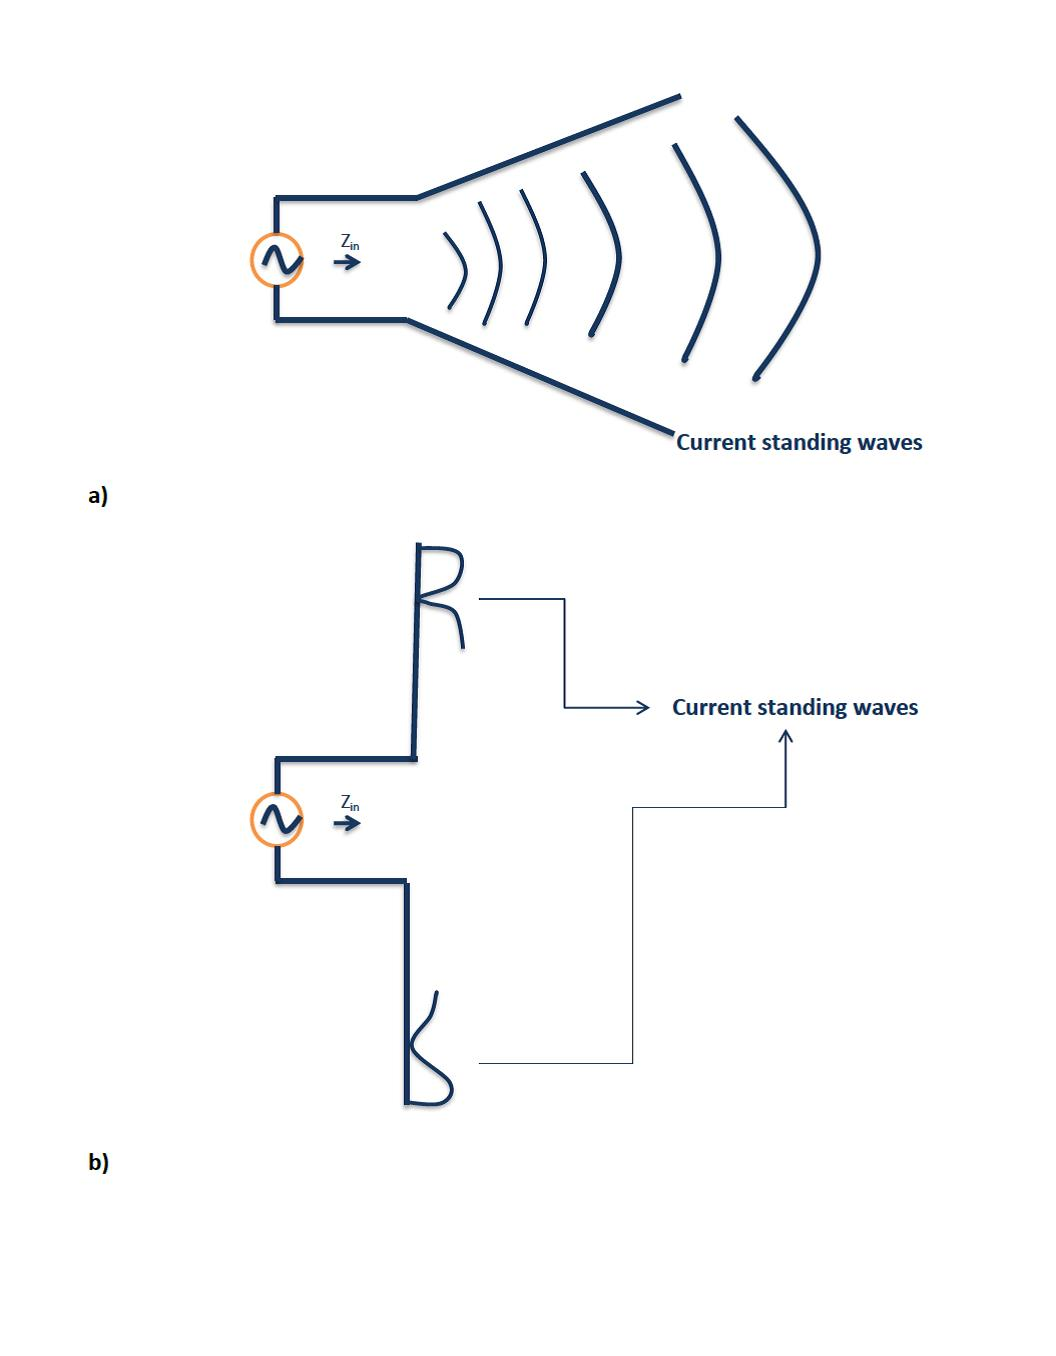
\includegraphics[height=5cm]{./graphics/fig_2}
\caption{Flared transmission line}
\end{figure}
Also we can take an extreme case and still have the nature of of standing wave retained in the TL when the ends are flared completely as shown in fig 1.3b. In this case the current distribution is in the same direction and is generating field which will not cancel each other.

While we would be discussing the topic, we would give answers to question like how much power is radiated and which direction would the power not be radiated. What kind of polarization will be developed by the structure? and so on.

Considering an antenna structure, we would say the structure has dual nature that is on one side, it acts as a circuit element with input impedance and bandwidth range, while on the other side it generates electric and magnetic fields with characteristics (in what direction does the wave propagate) and the power the fields radiate.
\begin{figure}
\centering
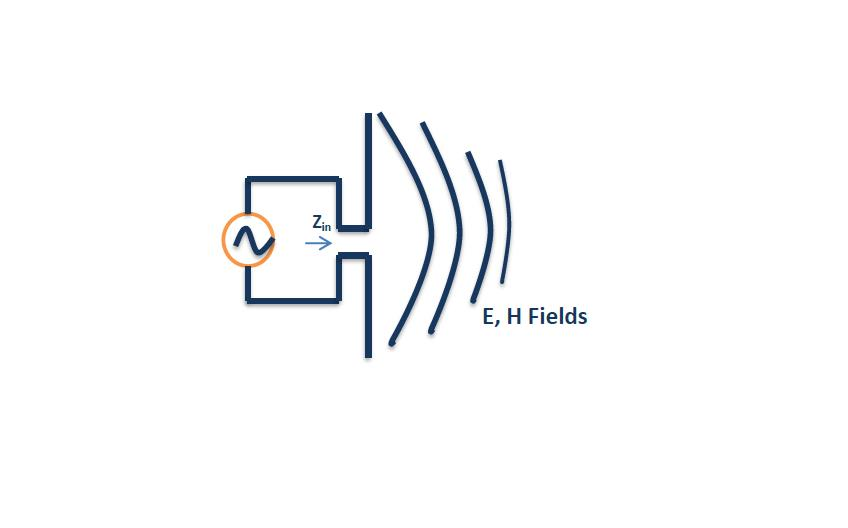
\includegraphics[height=5cm]{./graphics/fig_3}
\caption{Antenna characteristics}
\end{figure}

\begin{itemize}
\item \textbf{Circuit characteristics}
\item Input Impedance
\item Bandwidth
\end{itemize}

\begin{itemize}
\item \textbf{Wave Characteristics}
\item Kind of Polarization
\item Power Radiated
\item Directional Characteristics
\end{itemize}
Essentially, when investigating antennas, we consider the dual nature and concern ourselves with the input side when the antenna acts as a circuit element as well as treat it as a source of electromagnetic waves and provide their characteristics. 

\section{Mathematical Modeling of Radiation}
To model the problem of radiation, we refer back to Maxwell's Equation. In previous chapters, when modeling electromagnetic waves we considered both source free medium and a medium with finite conductivity. In a medium of finite conductivity we had conduction current density, but in this case we would separate these two medium when modeling radiation. One region would be the source region where there is current and charges and there is a different region where there would be the electric and magnetic fields.
\begin{figure}
\centering
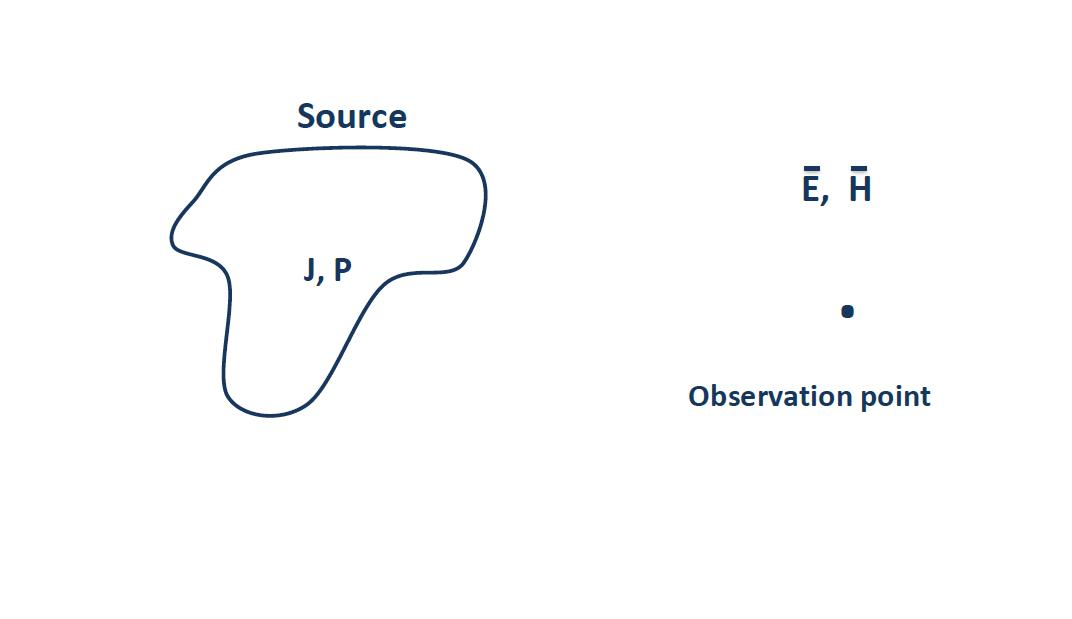
\includegraphics[height=5cm]{./graphics/fig_4}
\caption{Mathematical model}
\end{figure}

Lets consider a source of conduction current density $\vec{J}$ and volume charge density $\rho$ which produces electric and magnetic fields at some point called the observation point which source free as shown in Fig 1.5 The objective would be establishing the relationship between the electric and magnetic fields with the sources.

Some point to note in this analysis are;
\begin{itemize}
\item Previously when analyzing EM wave (the uniform plane wave) the source was pushed to infinity while here, the sources are at an observable distance from the point of reference.
\item When we analyzed the uniform plane wave we where not concerned with the choice of coordinate system to use and it was possible to model in the cartesian coordinate system which was an easier choice because the coordinates are not changing with direction but in this case the choice of coordinate system matters and the appropriate choice is the spherical coordinate system.
\end{itemize}

So the coordinate system normally used for antennas is the spherical coordinate system, as shown below

\begin{figure}
\centering
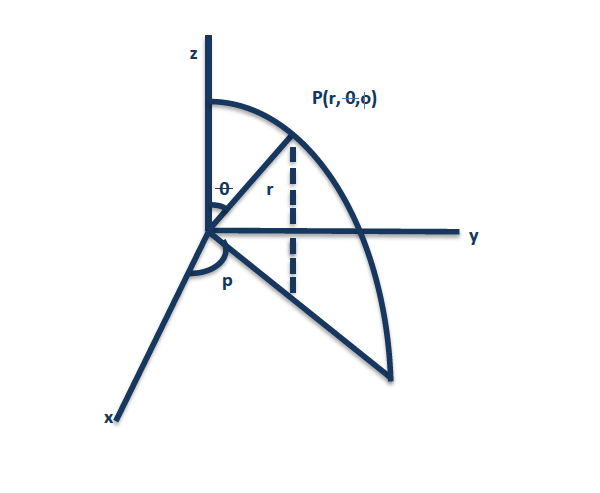
\includegraphics[height=5cm]{./graphics/fig_5}
\caption{Spherical coordinate}
\end{figure}

With that established lets reference the maxwell's equations given below
\begin{enumerate}
\item $$ \nabla\cdot\vec{D} =\rho\ or\ \nabla \cdot\vec{E} =\dfrac{\rho}{\epsilon} $$	
\item $$ \nabla\cdot\vec{B}=0$$	
\item $$\nabla\times\vec{E}=- \dfrac{\partial\vec{B}}{\partial t}$$
\item $$\nabla\times\vec{H}=\bar{J}+\dfrac{\partial\bar{D}}{\partial t}$$
\end{enumerate}

From (ii) $\nabla\cdot\vec{B}=0$ the condition is still satisfied, if it is rewritten as $\nabla\cdot(\nabla\times\vec{A})=0$, and we call the vector $\vec{A}$ the magnetic vector potential. Recall from the electrostatic case that calculating for the electric field for any problem was best approached by finding the scalar potential and this approach is applied here such that $\vec{B}=\nabla\times\vec{A}$ which simplifies the solution.

Our objectives are as follows
\begin{enumerate}
\item Find the solution for the potential A
\item Find the magnetic and electric fields and
\item Find the power radiated from the sources
\end{enumerate}

From (iii) $$\nabla\times\vec{E}=\dfrac{-\partial(\nabla\times\vec{A})}{\partial t}$$

interchanging the time and space derivatives gives
$$\nabla\times\vec{E}=-\nabla\times\dfrac{-\partial\vec{A}}{\partial t}$$

Let represent a time derivative with a dot ($\cdot$) on the vector
$$\nabla\times\vec{E}=-\nabla\times\dot{\vec{A}};$$

$$\nabla\times(\vec{E}+\dot{\vec{A}})=0;$$ Still the expression can be written as;

$$\vec{E}+\dot{\vec{A}}= -\nabla V$$ since $\nabla\times(-\nabla V)=0$

The minus sign is placed to retain the relationship between $\vec{E}$ and $V$. If the time varying magnetic scalar vector $\dot{\vec{A}}$ is removed from the expression

From (iv)
$\nabla\times\vec{H}=\vec{J}+\dot{\vec{D}}$
and $\vec{D}=\epsilon\vec{E}$

Then, $\nabla\times\vec{H}=\vec{J}+\epsilon\dot{\vec{E}}$ (we assume $\epsilon$ is not a function of time - a homogeneous medium)

From $\vec{B}=\nabla\times\vec{A}$, $\vec{B}=\mu\vec{H}$
\begin{equation}
\mu\vec{H}=\nabla\times\vec{A}
\end{equation}
\begin{equation}
\vec{H}=\dfrac{1}{\mu}\nabla\times\vec{A}
\end{equation}
Substitute equation 1.1 in 1.2 gives $$\nabla\times(\dfrac{1}{\mu}\nabla\times\vec{A})=\vec{J}+\epsilon\dot{\vec{E}}$$

Also $\mu$ is not a function of space (isotropic)

$$\nabla\times\nabla\times\vec{A}=\mu\vec{J}+\mu\epsilon\dot{\vec{E}}$$ 

Using vector identities
$$\nabla\times\nabla\times\vec{A}= \nabla(\nabla\cdot\vec{A}) -\nabla^{2}\vec{A}=\mu\vec{J}+\mu\epsilon\dot{\vec{E}}$$

Substituting $\dot{\vec{E}}=-(\nabla\dot{V}+\ddot{\vec{A}})$

$$\nabla(\nabla\cdot\vec{A}) -\nabla^{2}\vec{A}=\mu\vec{J}+\mu\epsilon(-(\nabla\dot{V}+\ddot{\vec{A}}))$$
$$=\mu\vec{J}+\mu\epsilon\nabla\dot{V}-\mu\epsilon\vec{A}$$ 
Rewriting the expression
\begin{equation}
\nabla^{2}\vec{A}-\mu\epsilon\ddot{\vec{A}}=-\mu\vec{J}+\mu\epsilon\nabla\dot{V}+\nabla(\nabla\cdot\vec{A})
\end{equation}


When the above expression is compared with the equation of electric and magnetic fields in a source free unbound medium (set $\vec{J}$ to zero for $\sigma=0$) It is seen that the above expression has the components $\mu\epsilon\nabla\dot{V}+\nabla(\nabla\cdot\vec{A})$ in addition to the equations of electric and magnetic fields in a source free unbounded medium given below
$$\nabla^{2}\vec{E}-\mu\epsilon\ddot{\vec{E}}=0$$
$$\nabla^{2}\vec{H}-\mu\epsilon\ddot{\vec{H}}=0$$


If these solutions satisfy the same boundary condition- it is source free and an unbound medium- then from the uniqueness theorem they are indeed the same solution. Hence we can make equation 1.3 unique by satisfying the uniqueness theorem and defining the expression for the divergence of the vector 'A'.

Hence, \begin{equation}
\mu\epsilon\nabla\dot{V}+\nabla(\nabla\cdot\vec{A})=0 \Rightarrow \nabla(\mu\epsilon\dot{V}+\nabla\cdot\vec{A})=0
\end{equation}

then
$$\nabla\cdot\vec{A}=-\mu\epsilon\dot{V}$$

which is called the Lorentz Gauge condition.
This condition defines the divergence of the magnetic vector potential
Now equation 1.3 reduces to
\begin{equation}
\nabla^{2}\vec{A}-\mu\epsilon\ddot{\vec{A}}=-\mu\vec{J}
\end{equation} 


Take the divergence of $\vec{E}+\dot{\vec{A}}=-\mu\vec{J}$ to give;

$$\nabla\cdot\vec{E}+\nabla\cdot\dot{\vec{A}}=-\nabla^{2} V$$\\
substituting	
$$\nabla\cdotp\dot{\vec{A}}=-\mu\epsilon\ddot{V}$$
$$\nabla\cdotp\vec{E}-\mu\epsilon\ddot{V}=-\nabla^{2} V$$

Rearranging; $\nabla^{2} V-\mu\epsilon\ddot{V}=-\nabla\cdotp\vec{E}$

From $\nabla\cdotp\vec{E}=\dfrac{\rho}{\epsilon}$, We get;
\begin{equation}
\nabla\dot\vec{E}-\mu\epsilon\ddot{V}=-\dfrac{\rho}{\epsilon}
\end{equation}

Both equations 1.5 and 1.6 can be rewritten as
\begin{center}
$\Box\vec{A}=\mu J$\\
$\Box V=\dfrac{\rho}{\epsilon}$\\
\end{center}
where $\Box$ is called the D'Alembertian Operator or box operator given by 

$$\Box=\dfrac{\partial^{2}}{\partial t^{2}}-\dfrac{1}{c^{2}}\nabla^{2}$$

With Lorentz gauge condition we get an identical solution to equation 1.6 for the scalar potential V. This expression shows that the magnetic vector potential is related to the conduction current density $\vec{J}$ and the scalar potential is related to the volume charge density $\rho$. In conclusion, when we have time varying sources, we would have electric potential and magnetic vector potential and both are essentially governed by the wave equation; which implies they have wave behaviour in the 3 dimensional space.